% !TeX root = ../../../main.tex

\begin{figure}
	\centering
	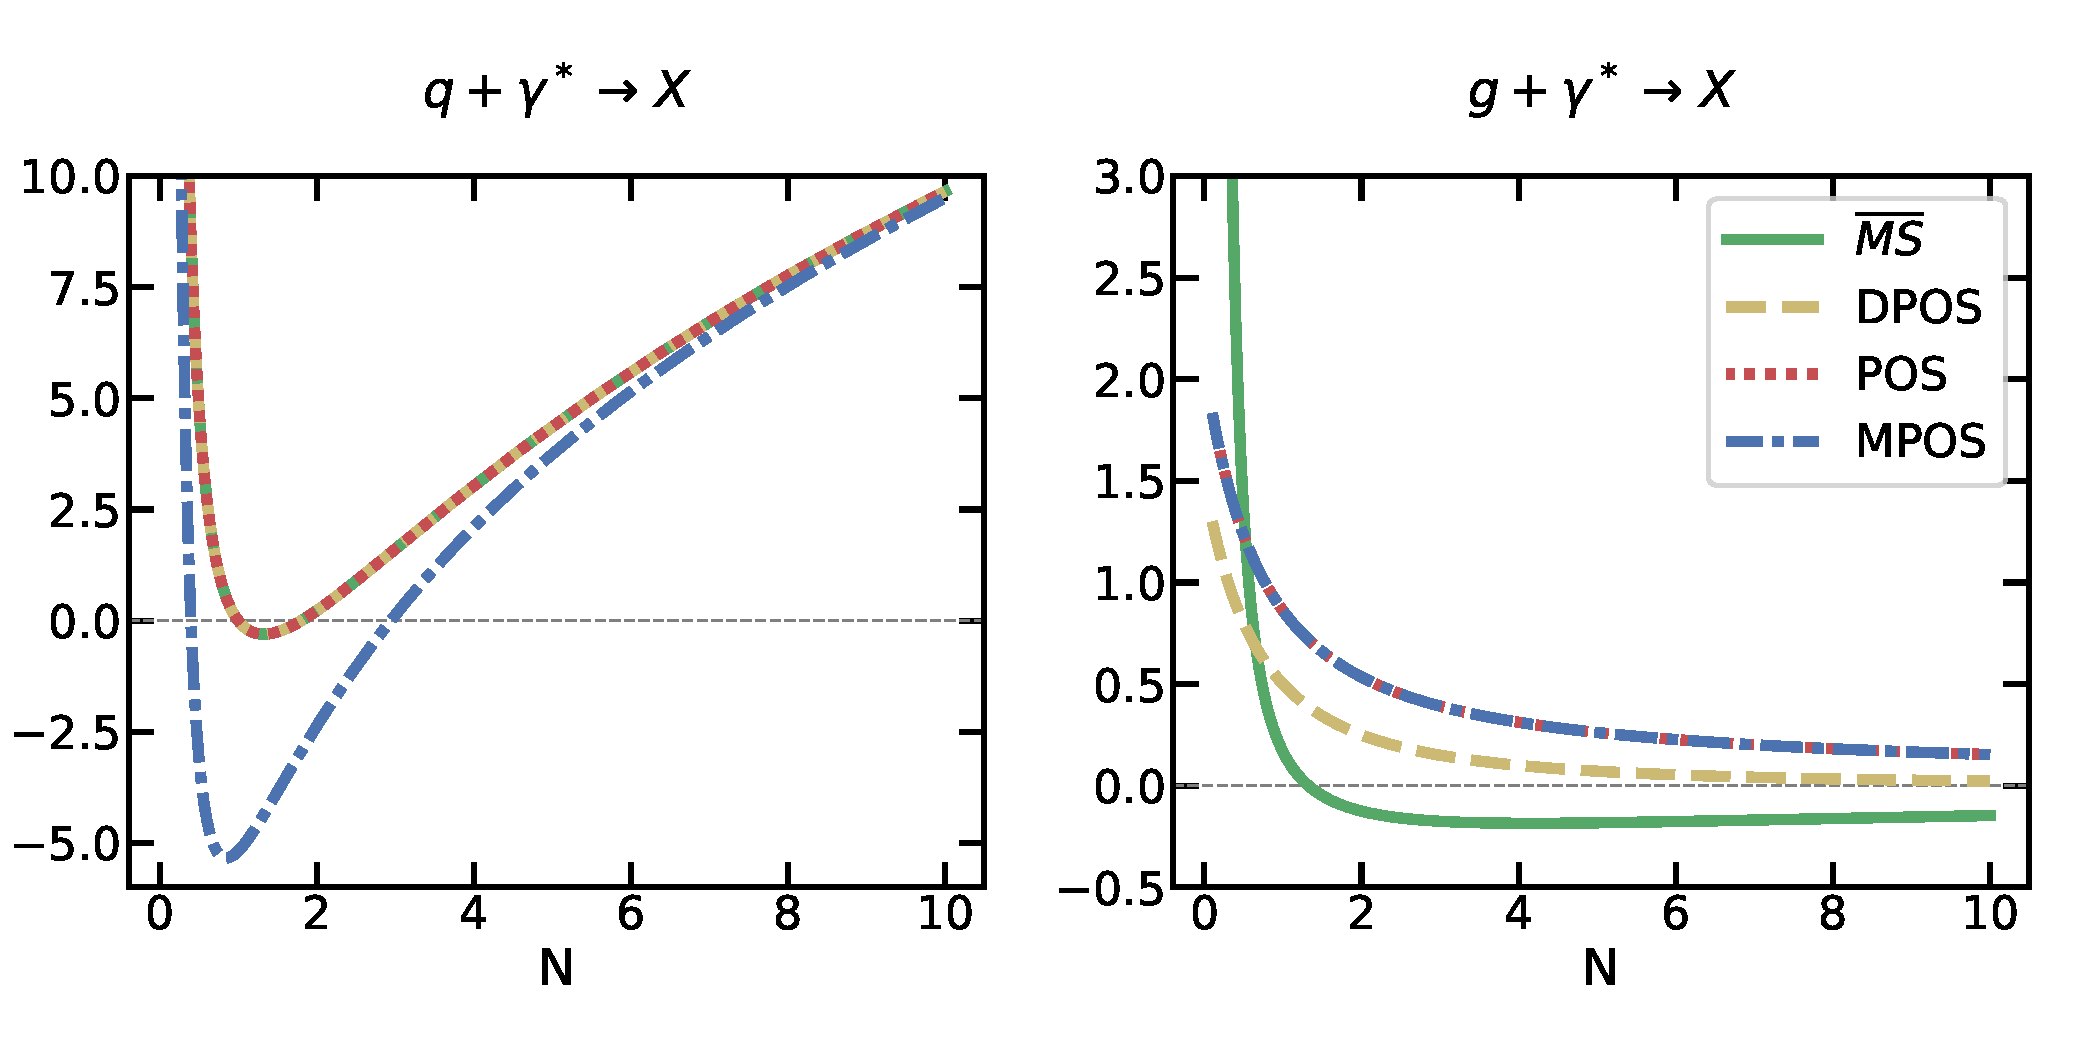
\includegraphics[width=0.7\textwidth]{ch-qcd/dis}
	\caption{
    The \lo Feynman diagram of the \dis process, including the original hadron.
    Kinematic variables indicated. Notice that, contrary to what is shown in
    the figure, in the text $x$ will be reserved for the hadronic Bjorken-$x$,
    while the partonic momentum fraction will usually be represented by $z$
    (the two of them coincide at this perturbative order).
  }
	\label{fig:dis/dis}
\end{figure}

\subsection{Kinematics}

The following variables are widely used to describe the kinematic of the \dis
process (cf. \cref{fig:dis/dis} for momenta definition):
\begin{itemize}
  \item $Q^2 = - q^2$ is the \ew boson virtuality (photon in the \acrshort{em}
    process)
  \item $M_h^2 = p^2$ the mass of the scattered hadron
  \item $\nu = q \cdot p$, mainly used in the definition of the following
  \item $x = \frac{Q^2}{2\nu}$, $y = \frac{q \cdot p}{k \cdot p}$ the Bjorken
    variables
\end{itemize}

\paragraph{Hadronic vs Partonic} Notice that the variables listed here
are all \textbf{hadronic}, so $x$ is not the partonic momentum fraction (it is only
at \lo , because the coefficient function is a Dirac $\delta$).
In order to avoid confusion the coefficient function variable will be called
$z$, and thus the partonic momentum fraction will be $x/z$.
\newline

It is possible to cut the \dis diagram on the exchanged boson, and compute
separately the two sides (cf.\ \cref{fig:dis/dis-lept-hadr}).
Since the boson is a Lorentz vector, it carries a space-time index, so the two
sides, once squared, will have two indices each, and for this reason they are
called the \textit{leptonic} and the \textit{hadronic tensors}.
%
At \lo in \ew corrections, the leptonic side does not couple to \qcd, so the
higher order corrections in the strong coupling are all on the side of the
hadronic tensor.
%
The fully inclusive \dis cross section $\sigma$ is thus given by
\begin{equation}
    \frac{d\sigma^i}{dx dy} = \frac{2\pi y \alpha^2}{Q^4} \sum_b \eta_b L^{\mu\nu}_b W_{\mu\nu}^b
\end{equation}
where $i \in \{\text{NC}, \text{CC}\}$ corresponds to the \nc or \cc processes,
respectively.
For \nc processes, the summation is over $b \in \{\gamma\gamma,\gamma Z,ZZ\}$,
whereas for \cc interactions there is only W exchange $b=\{W\}$.
The normalization factors $\eta_b$ denote the ratios of the corresponding
propagators and couplings to the photon propagator and coupling squared:
\begin{align}
    \eta_{\gamma\gamma} &= 1\\
    \eta_{\gamma Z} &= \frac{4\sin^2(\theta_w)}{1 - \sin^2(\theta_w)} \cdot \frac{Q^2}{Q^2 + M_Z^2}\\
    \eta_{ZZ} &= \eta_{\gamma Z}^2\\
    \eta_W &= \left(\frac{\eta_{\gamma Z}}{2} \frac{1 + Q^2/M_Z^2}{1 + Q^2/M_W^2}\right)^2
  \label{eq:dis/prop-corr}
\end{align}

\begin{figure}
	\centering
	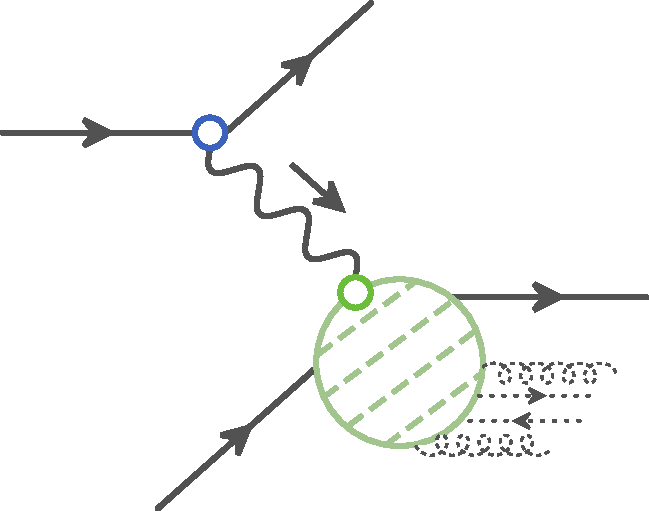
\includegraphics[width=0.6\textwidth]{ch-yadism/dis-hadronic-leptonic}
	\caption{
    In blue the leptonic coupling, the corresponding green one, close to the
    blob, is instead the hadronic coupling. The blob itself is the hadronic
    contribution.
  }
	\label{fig:dis/dis-lept-hadr}
\end{figure}

Based on symmetries and momenta involved, it is possible to characterize the
hadronic tensor with three scalar functions\footnote{
  This is true in the case of unpolarized \dis, while a few more functions have
  to be taken into account in the polarized case.
}:
\begin{align}
  W_{\mu\nu} =&~ \left(-g_{\mu\nu} + \frac{q_\mu q_\nu}{q^2}\right) F_1(x,Q^2)\nonumber\\
          &\qquad\qquad + \frac{\hat P_\mu \hat P_\nu}{P \cdot q} F_2(x,Q^2)\nonumber\\
          &\qquad\qquad\qquad\qquad - i \varepsilon_{\mu\nu\alpha\beta}
          \frac{q^\alpha P^\beta}{2 P\cdot q} F_3(x,Q^2)
  \label{eq:dis/hadr-tens}
\end{align}
with $\hat P_\mu = P_\mu - (P\cdot q / q^2) q_\mu$, $P$ the 4-momentum of the
hadron and $q$ the 4-momentum of the scattered boson.

These scalar functions are known as \dis \textit{structure functions}.

Instead, the leptonic tensors $L_b^{\mu\nu}$ can all be written in terms of the photonic
lepton tensor, because the lepton is assumed massless:
\begin{align}
    L^{\gamma\gamma}_{\mu\nu} &= 2\left(k_{\mu}k_{\nu}' + k_{\nu}k_{\mu}' - (k\cdot k') g_{\mu\nu} - i\lambda \epsilon_{\mu\nu\alpha\beta}k^{\alpha}k'^{\beta}\right)\\
    L^{b}_{\mu\nu} &= \kappa_b ~ L^{\gamma}_{\mu\nu}\\
    \kappa_{\gamma Z} &= (g_V^e + e\lambda g_A^e)\\
    \kappa_{ZZ} &= (g_V^e + e\lambda g_A^e)^2\\
    \kappa_{W} &= (1 + e\lambda)^2
\end{align}
with $g_V^e = -\frac 1 2 + 2\sin^2(\theta_w)$ and $g_A^e = -\frac 1 2$ the
vectorial and axial-vectorial coupling between the Z boson and the lepton with
charge $e=\pm 1$ and helicity $\lambda=\pm 1$.

Inserting the leptonic and the hadronic tensors into the cross section we obtain
\begin{align}
    \frac{d\sigma^i}{dx dy} = \frac{4\pi \alpha^2}{x y Q^2} \eta^i \left\{
    \left(1-y - \frac{x^2 y^2 M^2}{Q^2}\right)F_2^i
    + y^2 x F_1^i
    \pm \left(y - \frac {y^2}{2} \right) x F_3^i
    \right\}
\end{align}
where the $-$ sign in front of :math:$F_3$ is taken for an incoming $e^+$ or
$\bar \nu$ and the $+$ sign for an incoming $e^-$ or $\nu$.
The normalization factor $\eta^i$ are given by $\eta^{NC} = 1$ and $\eta^{CC} =
\kappa_W \eta_W$. So unlike in the \nc process, in the \cc process the leptonic
couplings and the propagator corrections are not inside the structure functions
but enter only on a cross section level. 
This is possible because in \cc there are no interferences between different bosons. 
The structure functions are given by
\begin{align}
    F_k^{CC} &= F_k^W\\
    F_k^{NC} &= F_k^{\gamma\gamma} - (g_V^e \pm \lambda g_A^e) \eta_{\gamma Z} F_k^{\gamma Z} \nonumber\\
             &\qquad + \left((g_V^e)^2 + (g_A^e)^2  \pm 2 \lambda g_V^e g_A^e \right) 
             \eta_{ZZ} F_k^{ZZ} \qquad~ k\in\{1,2,L\} \\
    x F_3^{NC} &= -(g_A^e \pm g_V^e) \eta_{\gamma Z} x F_3^{\gamma Z}
    + \left(2g_V^e g_A^e \pm \lambda((g_V^e)^2 + (g_A^e)^2)\right) x F_3^{ZZ}
\end{align}

\subsection{Process / Currents}

\dis is thought as a single process, but it can be drastically different
according to which \ew boson is actually exchanges.
It is actually possible to consistently define three different types of
possible \textbf{processes}, which correspond to a given \textit{set} of
scattering bosons:

\begin{itemize}
  \item \acrfull{ec}: the only boson allowed to be exchanged is the photon
  \item \acrfull{nc}: in addition to the photon, the $Z$ boson is also
    included, so this is a superset of \ec.
    Since now two bosons are allowed also interference terms appear.
    The $Z$ boson has an axial coupling to the leptons and thus it introduces
    the problems related to $\gamma_5$ \cite{Gnendiger:2017pys}.
    It is relevant to note that there are no \acrfull{fcnc} in the \sm, thus
    \nc will always conserve the incoming flavor
  \item \acrfull{cc}: only the $W^+$ \textit{or} $W^-$ are allowed to be
    exchanged.
    The actual boson is determined by the incoming scattering lepton and charge
    conservation. As the $W^\pm$ are flavor changing additional care is needed
    in the calculation.
\end{itemize}

The qualitative behavior of the three processes is drastically different,
especially \cc concerning flavor structure.
But at high energy also \nc predictions might be significantly different from
\ec, while at low scale the $Z$ contribution is mostly irrelevant.

\subsection{Structure Functions}

As noted above, there are three different structure functions, which we refer
to as different \textbf{kinds}.
Usually, we actually use a different choice for the basis of independent kinds,
with respect to what is shown above in \cref{eq:dis/hadr-tens}:

\begin{align}
    F_2,~ F_L = F_2 - 2xF_1,~ xF_3
\end{align}

Indeed, computing $F_L$ instead of $F_1$ is adventagous due to the Callan-Gross
relation \cite{Callan:1969uq} $F_L=0$ in the naive parton model.
Notice that the $F_L$ definition it is not always the one above, but it may be
corrected, since the actual $F_L$ is the object involved in Callan-Gross
relation, cf. \cref{sec:dis/fl-corrections}.
%
Even with this basis, $F_1$ is still available, but it is treated as a derived
quantity, as well as the total cross sections, that is coming from the
combination of all the structure functions in the hadronic tensor.

Moreover, the value of $xF_3$ is often preferred to the bare $F_3$ structure
function, to better represent the way it appears in the full cross section (its
\enquote{native scaling}).

Many experiments either quote the values of the computed structure functions,
as resolved by the reconstructed kinematics, or they prefer to report the value
of a \textit{reduced cross-section}, but there is not a unique definition for
it.
Several reduced cross-sections definitions, as defined by experimental
collaborations, are implemented and documented in \yadism.

Another level at which it is possible to split the \dis cross-section is the
flavor content of the diagrams involved.
By excluding different set of flavors it is possible to obtain what we call
different \textbf{heavynesses} for structure functions:
\begin{description}
  \item[total] this is the name we give, intuitively, to structure functions in
    which all possible contributions are taken into account (according to the
    chosen \acrlong{fns})
  \item[light] for these observables we deny all contributions by heavy quarks
    (exactly which quarks have to be considered massive depends once more on
    the \fns)
  \item[<heavy>] e.g.\ \textit{charm}, contains the contributions in which the
    heavy quark of selected flavor couples directly to the \ew boson (as if
    only the charge of the given flavor is non-zero, while all the other
    couplings are set to zero)
\end{description}

All the heavynesses are defined tuning parameters at Lagrangian level, e.g.\ by
imposing that the only the charm quark couples to \ew boson, setting to 0 all
the other couplings.
Because of this all the observables are potential physical observables, since
they are well-defined and free of divergences.

Notice that, as a consequence, the contributions in which the heavy quark is
present, but does not couple to the \ew boson, are not included nor in
\textit{light} neither in \textit{<heavy>}, but they are of course present in
\textit{total}, thus:
\begin{equation}
  O_{\text{total}} \neq O_{\text{light}} + \sum_{h \in \text{heavy}} O_h 
\end{equation}

